\chapter{Functional Breakdown of Selected Design}

\begin{figure}[h]
	\centering
	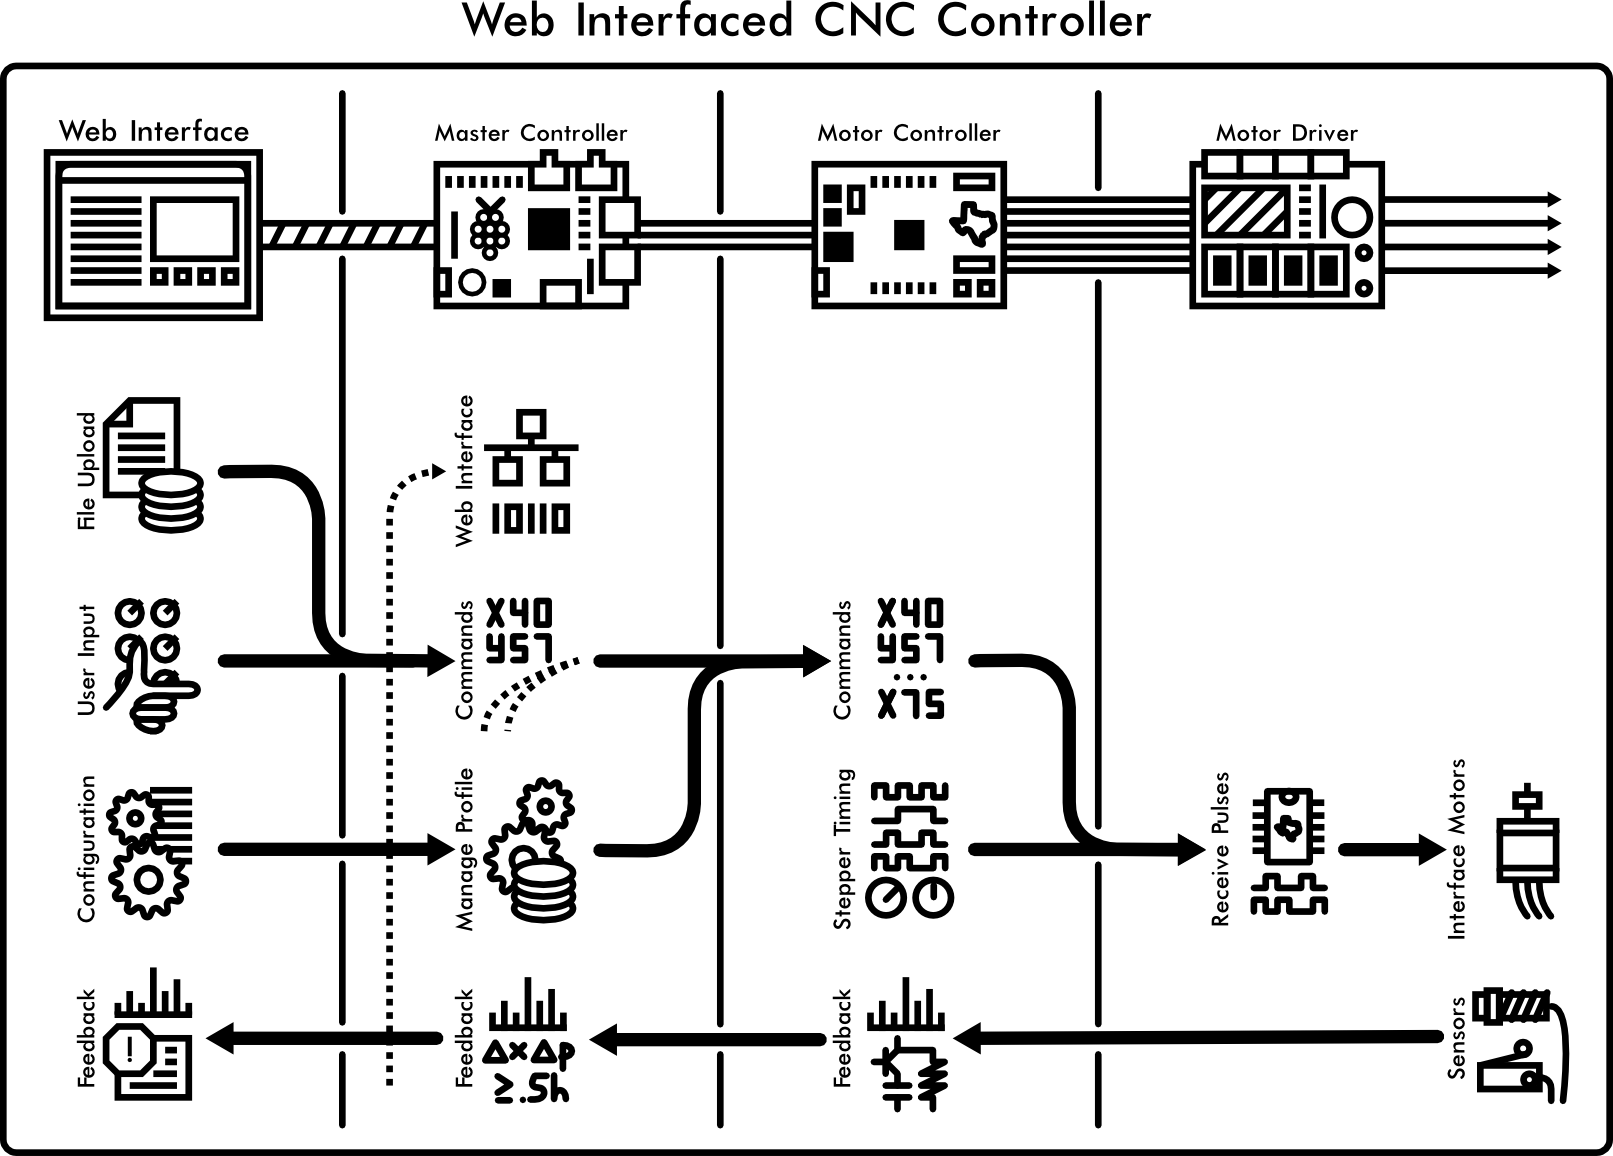
\includegraphics[width=1\textwidth]{architecture.png}
	\caption{System Architecture}
	\label{fig:architecture}
\end{figure}

\section{Level Zero Breakdown}
\begin{table}[H] 
	\caption{Zero Level Module Definition}
	\label{table:zerolevel}
	\centering 
	\begin{tabular}{|r p{10cm}|} 
		\hline\hline
		Module		& Web Interfaced CNC Controller \\ 
		Inputs		& User Commands \& Data files 	\\ 
		Outputs		& Motor Commands \& Feedback	\\ 
		Functionality	& This device will enable users to control CNC systems via a web-based interface 	\\ 
		\hline
		\end{tabular} 
\end{table}

\section{Level One Breakdown}
\begin{table}[H] 
	\caption{First Level Module Definition}
	\label{table:firstlevel}
	\centering 
	\begin{tabular}{|r p{10cm}|} 
		\hline\hline 
		Module		& Web Interface \\ 
		Inputs		& User Commands \& Data files, Master Control Feedback	\\ 
		Outputs		& Master Control Commands \& User Feedback \\ 
		Functionality	& This device will enable users to control CNC systems via a web-based interface by communicating with the Master Controller.\\ 
		\hline\hline 
		Module		& Master Control Board \\ 
		Inputs		& Master Control Commands \& Motor Controller Feedback	\\ 
		Outputs		& Motor Control Commands \& Web Interface Feedback \\ 
		Functionality	& This device will receive commands over the Internet, and interface them with the Motor Control Board. \\
		\hline\hline 
		Module		& Motor Control Board \\ 
		Inputs		& Motor Control Commands \& Sensor Feedback	\\ 
		Outputs		& Motor Driver Commands \& Master Controller Feedback \\ 
		Functionality	& This device will be responsible for realtime management of motor timing, and interfacing with the Motor Driver. It will also convert sensor feedback for the Master Control Board.\\
		\hline\hline 
		Module		& Motor Driver Board \\ 
		Inputs		& Motor Driver Commands \\ 
		Outputs		& Electronic control of Stepper Motors \\ 
		Functionality	& This device will manage the power and step-modes nessescary to manipulate the stepper motors based on the Motor Controller's commands. \\
		\hline\hline 
		Module		& Power Supply Unit \\ 
		Inputs		& Mains Voltage	\\ 
		Outputs		& Various Voltage Levels \\ 
		Functionality	& This device will manage power for the CNC Controller portion of the build. \\
		\hline
		\end{tabular} 
\end{table}

\section{Level Two Breakdown}
\begin{table}[H] 
	\caption{Second Level Module Definition - Web Interface}
	\label{table:secondlevelweb}
	\centering 
	\begin{tabular}{|r p{10cm}|} 
		\hline\hline 
		Module		& File Upload \\ 
		Inputs		& G-Code Files, Gerber Files, External Commands	\\ 
		Outputs		& Master Control Commands \\ 
		Functionality	& This unit will control conversion of User Data to Master Controller Commands.\\ 
		\hline\hline 
		Module		& Command Execution \\ 
		Inputs		& User Commands	\\ 
		Outputs		& Master Control Commands \\ 
		Functionality	& This unit will accept user commands (Left, Right, Stop) and convert them to the Master Controller Format.\\
		\hline\hline 
		Module		& Configure Machine \\ 
		Inputs		& User Input \\ 
		Outputs		& Master Control Commands \\ 
		Functionality	& This unit will be responsible for converting the User Machine Configuration information into Master Controller Commands.\\
		\hline\hline 
		Module		& Feedback Reception \\ 
		Inputs		& Master Controller Feedback \\ 
		Outputs		& User Feedback \\ 
		Functionality	& This unit will interpret feedback from the Master Controller, and present it to the end User. \\
		\hline
		\end{tabular} 
\end{table}

\begin{table}[H] 
	\caption{Second Level Module Definition - Master Control Board}
	\label{table:secondlevelmaster}
	\centering 
	\begin{tabular}{|r p{10cm}|} 
		\hline\hline 
		Module		& Web Interface \\ 
		Inputs		& Internet Data	\\ 
		Outputs		& Master Control Commands \\ 
		Functionality	& This unit will be responsible for interpreting data in the TCP/IP format for use as Master Control Commands.\\ 
		\hline\hline 
		Module		& Machine Profile Maintainence \\ 
		Inputs		& Master Control Commands (User Input)\\ 
		Outputs		& Local configuration settings \\ 
		Functionality	& This unit will store information about the CNC configuation locally for use in processing operations.\\
		\hline\hline  
		Module		& Command Processing \\ 
		Inputs		& Master Control Commands (User Commands \& G-Code etc.) \\ 
		Outputs		& Motor Control Commands \\ 
		Functionality	& This unit will calculate the desired course of action based off of the Machine Profile, and pass it to the Motor Controller.\\
		\hline\hline 
		Module		& Feedback Management \\ 
		Inputs		& Motor Controller Feedback \\ 
		Outputs		& Web Interface Feedback \\ 
		Functionality	& This unit will interpret feedback from the Motor Controller, and present it to the Web Interface. \\
		\hline
		\end{tabular} 
\end{table}

\begin{table}[H] 
	\caption{Second Level Module Definition - Motor Control Board}
	\label{table:secondlevelmotor}
	\centering 
	\begin{tabular}{|r p{10cm}|} 
		\hline\hline 
		Module		& Command Reception \\ 
		Inputs		& Motor Control Commands	\\ 
		Outputs		& Motor Driver Commands \\ 
		Functionality	& This unit will be responsible for processing position commands from the Master Controller.\\ 
		\hline\hline 
		Module		& Stepper Management \\ 
		Inputs		& Motor Control Commands \\ 
		Outputs		& Motor Driver Commands \\ 
		Functionality	& This unit will process the Motor Control Commands, and calculate the Step Frequency for real-time operation.\\
		\hline\hline  
		Module		& Feedback Management \\ 
		Inputs		& Sensor Feedback \\ 
		Outputs		& Master Controller Feedback \\ 
		Functionality	& This unit will interpret feedback from the Feedback Sensors, and present it to the Master Controller. \\
		\hline
		\end{tabular} 
\end{table}

\begin{table}[H] 
	\caption{Second Level Module Definition - Motor Driver Board}
	\label{table:secondleveldriver}
	\centering 
	\begin{tabular}{|r p{10cm}|} 
		\hline\hline 
		Module		& Command Reception \\ 
		Inputs		& Motor Driver Commands	\\ 
		Outputs		& Interface with Motor \\ 
		Functionality	& This unit will be responsible for allowing pulses from the Motor Control board to manipulate the Stepper Motors.\\
		\hline
		\end{tabular} 
\end{table}